\documentclass[12pt]{article}
\usepackage{amsmath,amssymb,bbold,bm,empheq,graphicx,hyperref,siunitx,subcaption,upgreek,xcolor}
\usepackage[a4paper, margin=1in]{geometry}
\usepackage[italicdiff]{physics}
\usepackage[justification=centering]{caption}
\usepackage{subcaption}
\usepackage[section]{placeins}

\hypersetup{colorlinks=true, urlcolor=cyan}
\newcommand{\ddfrac}[2]{{\displaystyle\frac{\displaystyle #1}{\displaystyle #2}}}

\title{FEM for Boltzmann Conductivity: An Introduction}
\author{Saleh Shamloo Ahmadi}

\begin{document}
\maketitle
\section{Problem Statement}
\subsection{The Boltzmann Transport Equation}
From the Boltzmann transport equation, we have
\begin{gather}
    \dv{f}{t} = \qty(\pdv{f}{t})_{\text{coll}}, \\
    \pdv{f}{t} + \frac{\vb{p}}{m}\vdot\grad_{\vb{r}} f + \vb{F}\vdot\grad_{\vb{p}}f = I[f],
\end{gather}
where $f$ is any density function, $\vb{p}$ is the momentum of the particles, $\vb{F}$ is the
external force, and $I[f]$ is the \emph{collision integral}. In the context of conductivity of
electrons,
\begin{equation}
    \vb{F} = -e\qty(\vb{E} + \vb{v}\cross\vb{B}),
\end{equation}
and replacing the momentum $\vb{p}$ with the wavevector $\vb{k}$, we have
\begin{equation}
    \pdv{f}{t} + \frac{\hbar\vb{k}}{m}\vdot\grad_{\vb{r}} f
    - \frac{e}{\hbar}\qty(\vb{E} + \vb{v}\cross\vb{B})\vdot\grad_{\vb{k}}f = I[f].
    \label{eq:boltzmann_general}
\end{equation}
If we consider a fluctuation to the equilibrium distribution $f_0(\vb{k})$ (the Fermi-Dirac
distribution here), then,
\begin{equation}
    f(\vb{r}, \vb{k}; t) = f_0(\vb{k}) + g(\vb{r}, \vb{k}; t)
\end{equation}
(assuming the material is uniform, the equilibrium distribution does not have any $\vb{r}$
dependence). We could also rewrite the wavevector gradient by applying the chain rule and using
the relation between the group velocity and the energy. That is,
\begin{empheq}[right={\empheqrbrace\implies\grad_{\vb{k}}
    f_0=\hbar\vb{v}\displaystyle\pdv{f_0}{\varepsilon}}]{align}
    \vb{v} &= \frac{\grad_{\vb{k}}\varepsilon}{\hbar} \\
    \grad_{\vb{k}}f_0 &= \qty(\grad_{\vb{k}}\varepsilon)\qty(\pdv{f_0}{\varepsilon}),
\end{empheq}
where $\vb{v}$ is the group velocity $\varepsilon$ is the energy. Using all this, equation
\eqref{eq:boltzmann_general} becomes
\begin{equation}
    \pdv{g}{t} + \frac{\hbar\vb{k}}{m}\vdot\grad_{\vb{r}} g
    - \frac{e(\vb{E} + \vb{v}\cross\vb{B})}{\hbar}\vdot\grad_{\vb{k}}g - I[f_0 + g]
    = e\vb{E}\vdot\vb{v}\pdv{f_0}{\varepsilon} \label{eq:boltzmann}
\end{equation}
(note that $\vb{v}\cross\vb{B}$ is perpendicular to $\vb{v}$). Now, we only consider the case of
uniform fields (i.e. no $\vb{r}$ dependence), so we can drop the spatial gradient term. Also, for
the conductivity tensor, we are only interested in the linear response to the electric field
$\vb{E}$, so we can drop the electric field term on the left-hand side ($g$ itself is in first order
with respect to the electric field, so multiplying by the electric field itself gives a term of
second order in the electric field). Finally, linearizing the collision integral in terms of the
fluctuation $g$, we have
\begin{equation}
    I[f_0 + g] = \int\dd{\vb{k'}} C(\vb{k}, \vb{k'}) g(\vb{k'}; t)
    - \int\dd{\vb{k'}} C(\vb{k'}, \vb{k}) g(\vb{k}; t) + \mathcal{O}(g^2),
\end{equation} 
where $C(\vb{k}, \vb{k'})$ is a scattering kernel. I call the two terms the \emph{in-scattering} and
\emph{out-scattering} terms respectively. The out-scattering is usually expressed with the
\emph{relaxation time} $\tau$ or \emph{scattering rate} $\Gamma=1/\tau$, which is equal to
\begin{equation}
    \frac{1}{\tau(\vb{k})} = \int\dd{\vb{k'}} C(\vb{k'}, \vb{k}).
\end{equation}

\sloppy{In-scattering is dropped in the \emph{relaxation time approximation}, which is the case for
the Chambers formula. Our goal here is to keep this term, as it especially becomes important when
there is strong anisotropy in the scattering, which is the case for cuprates. When the scattering
is roughly isotropic, $C(\vb{k}, \vb{k'})$ does not strongly depend on $\vb{k}$ and, because of
charge conservation,
$\int\dd{\vb{k'}} C(\vb{k}, \vb{k'}) g(\vb{k'}; t) \approx C\int\dd{\vb{k'}} g(\vb{k'}; t) = 0.$
Due to time-reversal symmetry, $C(\vb{k}, \vb{k'}) = C(\vb{k'}, \vb{k})$, so if we consider any
anisotropy in the out-scattering, we must do the same for the in-scattering. This means the
Chambers formula is just wrong for anisotropic scattering. So, why does it work effectively
anyway? The scattering in cuprates might only be low-angle, so the in-scattering is small compared
to the out-scattering.}

Plugging in the expression for the collision integral into equation \eqref{eq:boltzmann} and
applying the approximations, we get
\begin{equation}
    \qty(\pdv{t} + \frac{1}{\tau(\vb{k})} - \frac{e(\vb{v}\cross\vb{B})}{\hbar}\vdot\grad_{\vb{k}})
    g(\vb{k}; t) - \int\dd{\vb{k'}} C(\vb{k}, \vb{k'}) g(\vb{k'}; t)
    = e\vb{E}\vdot\vb{v}\pdv{f_0}{\varepsilon}.
\end{equation}
Depending on whether we want to study steady-state DC fields or AC fields, we can set $\pdv*{t}$ to
equal to zero or perform a Fourier transform and set $\pdv*{t} = -i\omega$. For the sake of
completeness, I will go with the latter case (just setting $\omega=0$ and using the regular,
non-Fourier-trasformed fields would produce the former case easily).

This equation can be expressed as
\begin{equation}
    \int \dd{\vb{k'}} v(\vb{k}) A(\vb{k}, \vb{k'}) g(\vb{k'}) = h(\vb{k})
    \label{eq:integral_equation}
\end{equation}
where
\begin{gather}
    A(\vb{k}, \vb{k'}) = \qty(-\frac{i\omega}{v(\vb{k})} + \frac{1}{v(\vb{k})\tau(\vb{k})}
        - \frac{e\qty(\vu{v}(\vb{k})\cross\vb{B})}{\hbar}\vdot\grad_{\vb{k}})\delta(\vb{k}-\vb{k'})
        - \frac{C(\vb{k},\vb{k'})}{v(\vb{k})}, \label{eq:operator} \\
    h(\vb{k}) = e\vb{E}\vdot\vb{v}(\vb{k})\pdv{f_0}{\varepsilon}.
\end{gather}
Where $v=\norm{\vb{v}}$ and $\vu{v}=\vb{v}/v$. Separating the velocity magnitude $v(\vb{k})$
seems like an arbitrary choice here, but it is done with good reason. Later, it will make the
formula for the conductivity tensor more symmetric and makes the calculation of $A$ a bit more
streamlined. The solution can be expressed as
\begin{equation}
    g(\vb{k}) = \frac{1}{v(\vb{k})} \int\dd{\vb{k'}} A^{-1}(\vb{k}, \vb{k'}) h(\vb{k'}).
\end{equation}
So, if we could discretize everything, this would just become a linear system of equations. This is
the goal of the finite element method (FEM).

\subsection{The Conductivity Tensor}
The current density is given by
\begin{equation}
    \vb{J} = -\frac{2e}{(2\pi)^d} \int_{\text{BZ}} \dd{\vb{k}} \vb{v}(\vb{k}) f(\vb{k}),
\end{equation}
where BZ is the Brillouin zone. The factor of 2 in the numerator is due to the two possible spin
configurations per wavevector $k$ and the factor $(2\pi)^d$ in the denominator comes from the
weighted sum over the wavevectors. The conductivity tensor is given by
\begin{equation}
    \sigma_{ab} = \pdv{J_a}{E_b}.
\end{equation}
Since there are no currents in equilibrium, we have
\begin{equation}
    \sigma_{ab} = -\frac{2e}{(2\pi)^d} \int_{\text{BZ}}\dd{\vb{k}} v_a(\vb{k}) \pdv{g(\vb{k})}{E_b}.
\end{equation}
plugging in the expression for $g(\vb{k})$,
\begin{equation}
    \sigma_{ab} = -\frac{2e^2}{(2\pi)^d} \int_{\text{BZ}}\dd{\vb{k}} \frac{v_a(\vb{k})}{v(\vb{k})}
    \int\dd{\vb{k'}} A^{-1}(\vb{k}, \vb{k'}) v_b(\vb{k'})\qty(\pdv{f_0}{\varepsilon}).
\end{equation}
As $T\to0$, the Fermi-Dirac distribution becomes a step function, so the term
$\pdv*{f_0}{\varepsilon}$ becomes a Dirac delta at the Fermi energy. If we apply the integral over
the delta function, an extra factor of $(\grad_{k}\varepsilon)^{-1} = (\hbar v)^{-1}$ (the Jacobian)
is added. In the end, we have
\begin{equation}
    \sigma_{ab} = -\frac{2e^2}{(2\pi)^d\hbar} \int_{\text{FS}}\dd{\vb{k}}\int\dd{\vb{k'}}
    \hat{v}_a(\vb{k}) A^{-1}(\vb{k}, \vb{k'}) \hat{v}_b(\vb{k'}),
    \label{eq:conductivity}
\end{equation}
where FS is the Fermi surface, and $\hat{v}_a=v_a/v$ is the component of the velocity in the
$a$ direction, divided by the full magnitude of the velocity.

\section{Finite Element Method}
\subsection{Discretization}
To solve this using the finite element method, we first define a set of basis functions, and then
approximate everything as a linear combination of these basis functions. So, the goal is to express
everything in equation \eqref{eq:conductivity} in terms of linear combinations of these basis
functions and transform the differential equation problem into a linear algebra problem. To do this,
we use the machinery of tensor calculus, but it is not necessary to have a deep understanding of it.
It is only used to simplify the notation.

Before we begin, remember the simple rule that when summing over an index, it should be on the top
for one quantity and on the bottom for another. If an index is not summed over, then it will
obviously stay where it is in the final quantity. We call this the \emph{index contraction} rule.
The placement of indices on the top or the bottom has a deeper connection with tensor calculus and
covariance and contravariance, but it is not needed to understand the procedures here. You can just
think of it as a syntactic game. I will also not use the Einstein summation convention, just to
make things completely explicit and hopefully clearer.

Defining the basis as the set $\{\psi_i(\vb{k})\}$, we can approximate any function by a linear
combination of these basis functions;
\begin{equation}
    f(\vb{k}) = \sum_i f^{i}\psi_i(\vb{k}). \label{eq:vector}
\end{equation}
Now, we would like to evaluate integrals over the Fermi surface. So, to make our notation simpler,
we can define quantities with subscripts to represent integrals. Also, notice these are projections
of the functions onto the basis functions.
\begin{equation}
    f_i \equiv \int\dd{\vb{k}} \psi_i(\vb{k}) f(\vb{k})
    = \sum_j f^j \int\dd{\vb{k}} \psi_i(\vb{k}) \psi_j(\vb{k})
    \label{eq:integral_vector}
\end{equation}
It is useful to define the quantity
\begin{equation}
    M_{ij} \equiv \int \dd{\vb{k}} \psi_i(\vb{k}) \psi_j(\vb{k}),
    \label{eq:overlap}
\end{equation}
which we call the \emph{overlap matrix}. Using it,
\begin{equation}
    f_i = \sum_j M_{ij} f^j.
    \label{eq:lowering_vector}
\end{equation}

We now try to define the operator in this basis. The question is, where should we put the indices
for the matrix representing the action of operator $A$ in this space? Well, the action of such
matrix on a vector $f^i$ should produce a new vector $(Af)^i$. This should be a linear combination
of the components of the vector $f^i$. So, to abide by our rule of index contraction, the symbol for
the matrix of $A$ should have one index on the bottom to sum over the elements of $f^i$ and one index
on the top for each of the elements of the resulting vector $(Af)^i$. Putting it all together,
\begin{equation}
    (Af)(\vb{k}) = \sum_i (Af)^i \psi_i(\vb{k}) \equiv \sum_{ij} A^i_j f^j \psi_i(\vb{k}).
\end{equation}
For the integrals, we have
\begin{equation}
    (Af)_i = \int\dd{\vb{k}} \psi_i(\vb{k}) (Af)(\vb{k}) = \sum_{jk} A^j_kf^k
    \int\dd{\vb{k}} \psi_i(\vb{k})\psi_j(\vb{k}) = \sum_{jk} M_{ij} A^j_k f^k.
    \label{eq:integral}
\end{equation}
To make it simpler, we can define the symbol
\begin{equation}
    A_{ij} \equiv \sum_k M_{ik} A^k_j
    \label{eq:lowering_matrix}
\end{equation}
so that
\begin{equation}
    (Af)_i = \sum_j A_{ij} f^j.
    \label{eq:integral_matrix}
\end{equation}

From equations \eqref{eq:lowering_vector} and \eqref{eq:lowering_matrix}, we can see that the
overlap matrix $M$ performs the action of \emph{lowering} the indices. If we invert this matrix
in each of these linear systems, we have
\begin{align}
    f^i &= \sum_j (M^{-1})^{ij} f_j, \\
    A^i_j &= \sum_k (M^{-1})^{ik} A_{kj}.
\end{align}
Again, the index placement is done by the index contraction rule. So we can see that the inverse of
the overlap matrix $M^{-1}$ performs the action of \emph{raising} the indices. In tensor algebra,
the equivalent of this is the metric tensor.

Finding the components of the vectors $f^i$ is easy; they are just the value of the functions at
each discrete point in our approximation space. But how do we find the elements of the matrix $A$?
The action of the operator $A$ on a function $f(\vb{k})$ is
\begin{equation}
    (Af)(\vb{k}) = \int\dd{\vb{k'}} A(\vb{k}, \vb{k'}) f(\vb{k'}).
\end{equation}
Inserting this into equation \eqref{eq:integral}, and utilizing equation \eqref{eq:integral_matrix},
we get
\begin{equation}
    \sum_j A_{ij} f^j = \int\dd{\vb{k}} \psi_i(\vb{k}) \int\dd{\vb{k'}} A(\vb{k}, \vb{k'}) f(\vb{k'}).
\end{equation}
expanding the function $f(\vb{k'})$ in terms of the basis functions from equation \eqref{eq:vector},
\begin{equation}
    \sum_j A_{ij} f^j = \int\dd{\vb{k}} \psi_i(\vb{k}) \int\dd{\vb{k'}} A(\vb{k}, \vb{k'})
    \sum_j f^j \psi_j(\vb{k'}).
\end{equation}
This is true for any function vector $f^j$, so we can drop it from both sides. This finally gives
\begin{equation}
    A_{ij} = \int\dd{\vb{k}} \int\dd{\vb{k'}} \psi_i(\vb{k}) A(\vb{k}, \vb{k'}) \psi_j(\vb{k'}).
    \label{eq:matrix_elements}
\end{equation}

Now that we know how to expand everything in this discrete basis, let us go back to our original
integral equation \eqref{eq:integral_equation}. We would like to solve
\begin{equation}
    \int \dd{\vb{k'}} A(\vb{k}, \vb{k'}) g(\vb{k'}) = (Ag)(\vb{k}) = h(\vb{k}).
\end{equation}
To express this equation in terms of the symbols we know, we can multiply both sides by
$\psi_i(\vb{k})$ and integrate over $\vb{k}$. This gives
\begin{equation}
    \int \dd{\vb{k}} \psi_i(\vb{k}) (Ag)(\vb{k}) = \int \dd{\vb{k}} \psi_i(\vb{k}) h(\vb{k}).
\end{equation}
Using equations \eqref{eq:integral_vector} and \eqref{eq:integral_matrix}, this becomes
\begin{equation}
    (Ag)_i = h_i.
\end{equation}
Expanding the left-hand side,
\begin{equation}
    \sum_j A_{ij} g^j = h_i
\end{equation}
and solving the linear system,
\begin{equation}
    g^i = \sum_j (A^{-1})^{ij} h_j.
    \label{eq:inverse}
\end{equation}
Again, the index placement is done by the index contraction rule. The important result is that
we need to invert the $A_{ij}$ form of the matrix to get the inverse we need for our case.
\begin{equation}
    (A^{-1})^{ij} = (A_{ij})^{-1}.
\end{equation}

Finally, to calculate the conductivity tensor from \eqref{eq:conductivity}, we need to multiply
$\hat{v}_a$ with $A^{-1}\hat{v}_b$ and take an integral over the result. To express this operation
in our discrete basis, consider two functions $f$ and $g$. Their product is
\begin{equation}
    f(\vb{k})g(\vb{k}) = \sum_{ij} f^i g^j \psi_i(\vb{k}) \psi_j(\vb{k}),
\end{equation}
and the integral over this product is
\begin{equation}
    \int\dd{\vb{k}} f(\vb{k}) g(\vb{k}) = \sum_{ij} f^i g^j \int\dd{\vb{k}}
    \psi_i(\vb{k})\psi_j(\vb{k}) = \sum_{ij} f^i g^j M_{ij} = \sum_i f^i g_i.
\end{equation}
So, the vector for one function needs to have indices on top and the other on the bottom. From
equation \eqref{eq:inverse}, we can see $A^{-1}\hat{v}_b$ has the form
$(A^{-1})^{ij} (\hat{v}_b)_j$, which would have an index on top after contraction. Therefore,
$\hat{v}_a$ would have to have an index on the bottom to perform the multiplication and integration.

Putting everything together, we have
\begin{equation}
    \sigma_{ab} = -\frac{2e^2}{(2\pi)^d\hbar} \sum_{ij} \qty(\hat{v}_a)_i
    \qty(A^{-1})^{ij} \qty(\hat{v}_b)_j,
\end{equation}
or, in terms of all the terms we know how to calculate,
\begin{equation}
    \sigma_{ab} = -\frac{2e^2}{(2\pi)^d\hbar} \sum_{ij} \qty[
    \qty(\sum_k M_{ik} (\hat{v}_a)^k) \qty(A_{ij})^{-1} \qty(\sum_k M_{jk} \qty(\hat{v}_b)^k)].
\end{equation}
To do the computation in practice, $M_{ij}$ and $A_{ij}$ can be calculated from \eqref{eq:overlap}
and \eqref{eq:matrix_elements} respectively, and $(\hat{v}_a)^i$ and $(\hat{v}_b)^i$ vector
components are the values of $\hat{v}_a$ and $\hat{v}_b$ at the discrete points of our approximation
space.  Afterwards, all that will be left to do is two matrix multiplications $M\hat{v}$, one linear
system solution $A^{-1}(M\hat{v}_b)$, and one dot product $(M\hat{v}_a)\vdot(A^{-1}M\hat{v}_b)$.

\subsection{Differential Operator Terms}
Splitting $A$ into the comprising terms using \eqref{eq:operator} and \eqref{eq:matrix_elements},
we have
\begin{align}
A_{ij} &= \begin{aligned}[t]
    &\int\dd{\vb{k}} \qty(-i\omega + \frac{1}{\tau(\vb{k})})
        \frac{\psi_i(\vb{k})\psi_j(\vb{k})}{v(\vb{k})} \\
    &-\int\dd{\vb{k}} \psi_i(\vb{k})\frac{e\qty(\vu{v}(\vb{k})\cross\vb{B})}{\hbar}
        \vdot\grad_{\vb{k}}\psi_j(\vb{k}) \\
    &- \int\dd{\vb{k}} \int\dd{\vb{k'}}
    \psi_i(\vb{k}) \frac{C(\vb{k},\vb{k'})}{v(\vb{k})} \psi_j(\vb{k'})
\end{aligned} \\
&\equiv \Gamma_{ij} - \frac{eB}{\hbar} \qty(D_{\vu{v}\cross\vu{B}})_{ij} - S_{ij}.
\end{align}
The matrices $\Gamma_{ij}$, $D_{\vu{v}\cross\vu{B}}$ and $S_{ij}$ are called the
\emph{out-scattering}, \emph{derivative} and \emph{in-scattering} matrices respectively.

Expanding the $k$-dependence in terms of the basis functions for the out-scattering
matrix $\Gamma_{ij}$ gives
\begin{equation}
    \Gamma_{ij} = \sum_k \int\dd{\vb{k}} \qty(-i\omega + \frac{1}{\tau_k})
    \frac{\psi_i(\vb{k})\psi_j(\vb{k})\psi_k(\vb{k})}{v_k}.
\end{equation}
Let us define the tensor $\Pi_{ijk}$ and the vector $\gamma^k$, such that
\begin{empheq}[left={\Gamma_{ij}=\sum_k\Pi_{ijk}\gamma^k\implies\empheqlbrace}]{align}
    \Pi_{ijk} &= \int\dd{\vb{k}} \psi_i(\vb{k})\psi_j(\vb{k})\psi_k(\vb{k}), \\
    \gamma^k &= -\frac{i\omega}{v_k} + \frac{1}{v_k\tau_k}.
\end{empheq}
So, for any given basis, we have to calculate the $\Pi_{ijk}$ tensor. The $\gamma^k$ vector
is given by the velocity, frequency, and scattering kernel (or possibly the scattering rate
$1/\tau$ defined ``by hand'' when ignoring in-scattering).

Expanding the $k$-dependence in terms of the basis functions for the in-scattering matrix $S_{ij}$
gives
\begin{equation}
    S_{ij} = \sum_{mn} \int\dd{\vb{k}} \int\dd{\vb{k'}} \psi_i(\vb{k})\psi_m(\vb{k})
    \frac{C_{mn}}{v_m}\psi_n(\vb{k'})\psi_j(\vb{k'}).
\end{equation}
Let us define the tensor $\Xi_{ijmn}$ and the matrix $s^{mn}$, such that
\begin{empheq}[left={S_{ij}=\sum_{m,n}\Xi_{ijmn}s^{mn}\implies\empheqlbrace}]{align}
    \Xi_{ijmn} &= \int\dd{\vb{k}} \int\dd{\vb{k'}} \psi_i(\vb{k})\psi_j(\vb{k'})
    \psi_m(\vb{k})\psi_n(\vb{k'}), \\
    s^{mn} &= \frac{C_{mn}}{v_m}.
\end{empheq}
So, for any given basis, we have to calculate the $\Xi_{ijmn}$ tensor and the $s^{mn}$ matrix
is given from the scattering kernel.

\subsection{Piecewise Linear Basis for 2D Fermi Surfaces}
The 2D case is a bit simpler and can help you gain a better understanding before moving to the
full 3D case.

We choose $n$ points on $\vb{k}_i$ to represent the Fermi surface. Then, the discretization of the
Fermi surface would be the line segments $I_i$ connecting these points. These line segments are also
called the \emph{elements}. The length of each line segment is
\begin{equation}
    \ell_i = \abs{\vb{k}_{i+1} - \vb{k}_i}.
\end{equation}
Note that since our domain is a closed curve (the Fermi surface is closed), there are periodic
boundary conditions, which means the point $i=n+1$ is the same as $i=1$ and $i=0$ is the same as
$i=n$. The simplest continuous basis one can define on these elements is the piecewise linear basis.
The basis function for each point $\vb{k}_i$ on the Fermi surface is linear on the connected
elements and peaks at the point $\vb{k}_i$, equal to 1. It is zero everywhere else. So, with the
parametrization of each line segment $I_i$ as
\begin{equation}
    x: I_i \mapsto [0, 1],
\end{equation}
then the basis functions can be defined as
\begin{empheq}[left={\psi_i(\vb{k})=\empheqlbrace}]{align}
    &x,& &\vb{k} \in I_{i-1}; \\
    &1-x,& &\vb{k} \in I_i; \\
    &0,& &\vb{k} \in I_j,\ j\notin \{i-1,i\}.
\end{empheq}

We can now calculate the matrices $M_{ij}$ and $A_{ij}$ in this basis. It is easy to see that, because
each element in these matrices contains the multiplication of two basis functions, they are only
nonzero when $i$ and $j$ are associated with the same point or neighboring points.

For the overlap matrix,
\begin{equation}
\begin{aligned}
    M_{ii} &= \int\dd{k}\psi_i(\vb{k})\psi_i(\vb{k}) = \int_{I_{i-1}} \dd{\vb{k}}
    \qty[\psi_i(\vb{k})]^2 + \int_{I_i} \dd{\vb{k}} \qty[\psi_i(\vb{k})]^2\\
    &= \int_0^1 \dd{x} x^2 \ell_{i-1} + \int_0^1 \dd{x} (1-x)^2 \ell_i
    = \frac{\ell_{i-1} + \ell_i}{3},
\end{aligned}
\end{equation}
\begin{equation}
    M_{i,i+1} = M_{i+1,i} = \int_{I_i} \dd{\vb{k}} \psi_i(\vb{k})\psi_{i+1}(\vb{k})
    = \int_0^1 \dd{x} x(1-x) \ell_i = \frac{\ell_i}{6}.
\end{equation}
Therefore, the full overlap matrix is
\begin{equation}
    M_{ij} = \frac{\ell_{i-1} + \ell_i}{3}\delta_{ij}
    + \frac{\ell_i}{6}\qty(\delta_{i+1,j} + \delta_{i,j+1}).
\end{equation}

For the derivative term $D_{\vu{v}\cross\vu{B}}$, note that the part
\begin{equation}
    (\vu{v}(\vb{k})\cross\vu{B})\vdot\grad_{\vb{k}}
\end{equation}
is the directional derivative in the direction $\vu{v}(\vb{k})\cross\vu{B}$. Since the functions are
only defined on the discretized 2D rings in $k$-space, this is the dot product of the vector
$\vu{v}(\vb{k})\cross\vu{B}$ with the direction of the vector $\vb{k}_{i+1} - \vb{k}_i$ (which is
along the line segment $I_i$), which we call $\Delta\vu{k}_i$. The diagonal terms vanish, since the
integral over $I_i$ and $I_{i-1}$ are completely the same, but with opposite signs; in the
direction of $\vb{k}_{i-1}$ to $\vb{k}_i$, the function $\psi_i$ increases on $I_{i-1}$, and in the
direction of $\vb{k}_i$ to $\vb{k}_{i+1}$, it decreases on $I_i$. The neighboring terms are
\begin{equation}
\begin{aligned}
    \qty(D_{\vu{v}\cross\vu{B}})_{i,i+1} &= -\qty(D_{\vu{v}\cross\vu{B}})_{i+1,i}
        = \int_{I_i} \dd{\vb{k}} \psi_i(\vb{k})
        \frac{\qty(\vu{v}_i\cross\vu{B})\vdot\Delta\vu{k}_i}{\ell_i} \\
    &= \int_0^1 \dd{x} (1-x) \qty[\qty(\vu{v}_i\cross\vu{B})\vdot\Delta\vu{k}_i]
    = \frac{\qty(\vu{v}_i\cross\vu{B})\vdot\Delta\vu{k}_i}{2},
\end{aligned}
\end{equation}
So, the full matrix is
\begin{equation}
    \qty(D_{\vu{v}\cross\vu{B}})_{ij} = \qty(\vu{v}_i\cross\vu{B})\vdot\Delta\vu{k}_i
    \qty(\frac{\delta_{i,j+1} - \delta_{i+1,j}}{2}).
\end{equation}

For the out-scattering term $\Gamma_{ij}=\sum_k\Pi_{ijk}\gamma^k$, only the elements where $i$, $j$ and $k$ are all
associated with the same point or neighboring points are nonzero.
\begin{equation}
    \Pi_{iii} = \int_{I_i} \dd{\vb{k}} \qty[\psi_i(\vb{k})]^3 + \int_{I_{i-1}}
        \dd{\vb{k}} \qty[\psi_i(\vb{k})]^3
    = \int_0^1 \dd{x} x^3 \ell_i + \int_0^1 \dd{x} (1-x)^3 \ell_{i-1}
    = \frac{\ell_i + \ell_{i-1}}{4},
\end{equation}
\begin{equation}
    \Pi_{i+1,i,i} = \Pi_{i,i+1,i} = \Pi_{i,i,i+1} = \int_{I_i} \dd{\vb{k}}
    \qty[\psi_i(\vb{k})]^2\psi_{i+1}(\vb{k}) = \int_0^1 \dd{x} (1-x)^2 x \ell_i = \frac{\ell_i}{12},
\end{equation}
\begin{equation}
    \Pi_{i,i+1,i+1} = \Pi_{i+1,i,i+1} = \Pi_{i+1,i+1,i} = \int_{I_i} \dd{\vb{k}}
    \psi_i(\vb{k})\qty[\psi_{i+1}(\vb{k})]^2 = \int_0^1 \dd{x} x(1-x)^2 \ell_i = \frac{\ell_i}{12},
\end{equation}
\begin{equation}
    \Pi_{ijk} = \frac{\ell_{i-1} + \ell_i}{4}\delta_{ijk}
    + \frac{\ell_i}{12}\qty(\delta_{i+1,j,k} + \delta_{i,j-1,k})
    + \frac{\ell_j}{12}\qty(\delta_{i,j+1,k} + \delta_{i,j,k-1})
    + \frac{\ell_k}{12}\qty(\delta_{i,j,k+1} + \delta_{i-1,j,k})
\end{equation}
Multiplying this tensor by $\gamma^k$, we get the full $\Gamma_{ij}$ matrix.
\begin{equation}
\begin{aligned}
    \Gamma_{ij} = \qty(\frac{\ell_{i-1} + \ell_i}{4}\gamma^i + \frac{\ell_i}{12}\gamma^{i+1}
        + \frac{\ell_{i-1}}{12}\gamma^{i-1})\delta_{ij}
    &+ \frac{\ell_i}{12}\qty(\gamma^i + \gamma^{i+1})\delta_{i+1,j} \\
    &+ \frac{\ell_j}{12}\qty(\gamma^j + \gamma^{j+1})\delta_{i,j+1}
\end{aligned}
\end{equation}

\subsection{Piecewise Linear Basis for 3D Fermi Surfaces}
The discretization procedure for the 3D case can be a bit more complicated. In addition to points,
we also need to define some connecting surface for sets of points. In 2D, this was easy because we
could just connect pairs of points with line segments. In 3D, to make the elements as simple as
possible, we use triangles.

We define the Fermi surface by a set of points $\vb{k}_i$ and triangles $T(i,j,k)$ connecting the
points $\vb{k}_i$, $\vb{k}_j$ and $\vb{k}_k$. Also, we define $T_i$ as the set of triangles
containing the point $\vb{k}_i$. Then, defining piecewise linear basis functions, the basis function
$\psi_i$ peaks with value 1 at the point $\vb{k}_i$, is linear on $T_i$, and is 0 everywhere else.

Each triangle is parametrized as
\begin{equation}
    (x, y): T(i,j,k) \mapsto \{(x, y);\; x\in[0, 1],\, y\in[0, 1-x] \},
\end{equation}
so that each triangle is mapped to a unit right-angled triangle.
With this mapping, the basis functions can be defined as
\begin{empheq}[left={\psi_i(\vb{k})=\empheqlbrace}]{align}
    &1 - x - y,& &\vb{k} \in T_i, (x, y)_{\max(\psi_i)} = (0, 0); \\
    &x,& &\vb{k} \in T_i, (x, y)_{\max(\psi_i)} = (1, 0); \\
    &y,& &\vb{k} \in T_i, (x, y)_{\max(\psi_i)} = (0, 1); \\
    &0,& &\vb{k} \notin T_i.
\end{empheq}
To visualize these basis functions more easily, you can look at Figure
\ref{fig:triangular_element}.

\begin{figure}
    \centering
    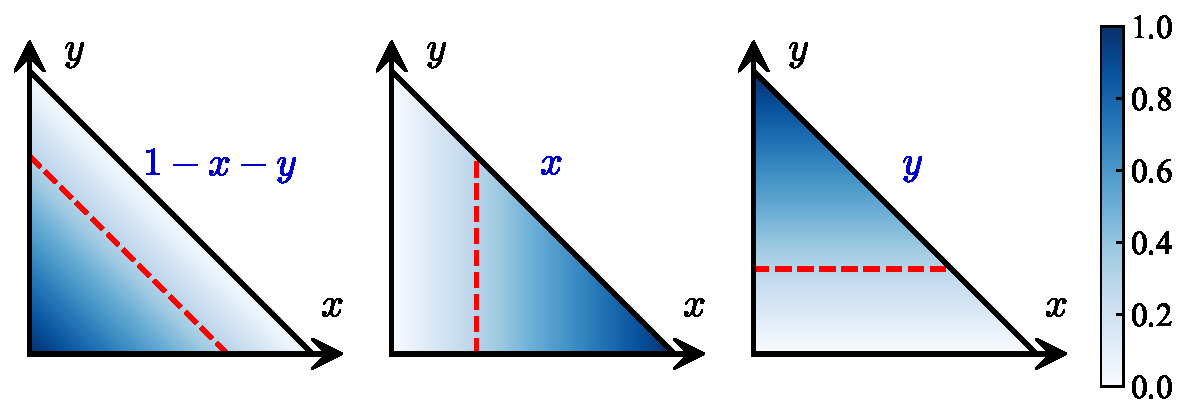
\includegraphics[width=\textwidth]{figures/triangular_element}
    \caption{visualization of the basis functions when the function peaks at each of the three
        vertices of the triangle.}
    \label{fig:triangular_element}
\end{figure}

To compute integrals with this parametrization, we can just use the Jacobian of the transformation.
Here, the Jacobian is the ratio of the area of the triangle $T(i,j,k)$ to the area of the unit
right-angled triangle. Let us define it as
\begin{equation}
    \alpha(i,j,k)=\norm{(\vb{k}_j - \vb{k}_i) \times (\vb{k}_k - \vb{k}_i)}.
\end{equation}
Then, the integrals are transformed as
\begin{equation}
    \int_{T(i,j,k)} \dd{\vb{k}} = \alpha(i,j,k)\int_0^1\dd{x}\int_0^{1-x}\dd{y}
    \equiv \alpha(i,j,k)\int_T\dd{x}\dd{y}.
\end{equation}

Now, for calculating each term, note that only the elements where the indices are the same or belong
to the same triangle have nonzero overlap (see Figure \ref{fig:triangle_overlap}). Here are all the
nonzero terms in the matrices:
\begin{align}
M_{ii} &= \int\dd{\vb{k}}\psi_i(\vb{k})\psi_i(\vb{k})
    = \sum_{(i,j,k) \in T_i} \int_{T(i,j,k)} \dd{\vb{k}} (\psi_i(\vb{k}))^2 \\
    &= \sum_{(i,j,k) \in T_i} \alpha(i,j,k) \int_T \dd{x} \dd{y} (1 - x - y)^2
    = \frac{1}{12} \sum_{(i,j,k) \in T_i} \alpha(i,j,k), \notag \\
M_{ij} &= \int\dd{\vb{k}}\psi_i(\vb{k})\psi_j(\vb{k})
    = \sum_{(i,j,k) \in T_i \cap T_j} \int_{T(i,j,k)} \dd{\vb{k}} \psi_i(\vb{k}) \psi_j(\vb{k}) \\
    &= \sum_{(i,j,k) \in T_i \cap T_j} \alpha(i,j,k) \int_T \dd{x} \dd{y} (1 - x - y)x
    = \frac{1}{24} \sum_{(i,j,k) \in T_i \cap T_j} \alpha(i,j,k) \notag \\
    \left(\vphantom{\sum_{(i)}}\right. &=\left.\sum_{(i,j,k) \in T_i \cap T_j}
    \alpha(i,j,k) \int_T \dd{x} \dd{y} (1 - x - y)y \right) \notag
\end{align}
\begin{align}
\Pi_{iii} &= \int\dd{\vb{k}}\psi_i(\vb{k})\psi_i(\vb{k})\psi_i(\vb{k})
    = \sum_{(i,j,k) \in T_i} \int_{T(i,j,k)} \dd{\vb{k}} (\psi_i(\vb{k}))^3 \\
    &= \sum_{(i,j,k) \in T_i} \alpha(i,j,k) \int_T \dd{x} \dd{y} (1 - x - y)^3
    = \frac{1}{20} \sum_{(i,j,k) \in T_i} \alpha(i,j,k), \notag \\
\Pi_{iij} &= \Pi_{iji} = \Pi_{jii} = \int\dd{\vb{k}}\psi_i(\vb{k})\psi_i(\vb{k})\psi_j(\vb{k})
    = \sum_{(i,j,k) \in T_i \cap T_j} \int_{T(i,j,k)} \dd{\vb{k}}
        (\psi_i(\vb{k}))^2 \psi_j(\vb{k}) \\
    &= \sum_{(i,j,k) \in T_i \cap T_j} \alpha(i,j,k) \int_T \dd{x} \dd{y} (1 - x - y)^2 x
    = \frac{1}{60} \sum_{(i,j,k) \in T_i \cap T_j} \alpha(i,j,k), \notag\\
\Pi_{ijk} &= \int_{T(i,j,k)} \dd{\vb{k}}\, \psi_i(\vb{k}) \psi_j(\vb{k}) \psi_k(\vb{k})
= \alpha(i,j,k) \int_T \dd{x} \dd{y} (1 - x - y)xy = \frac{1}{120} \alpha(i,j,k).
\end{align}

\begin{figure}
    \centering
    \begin{subfigure}{0.49\linewidth}
        \centering
        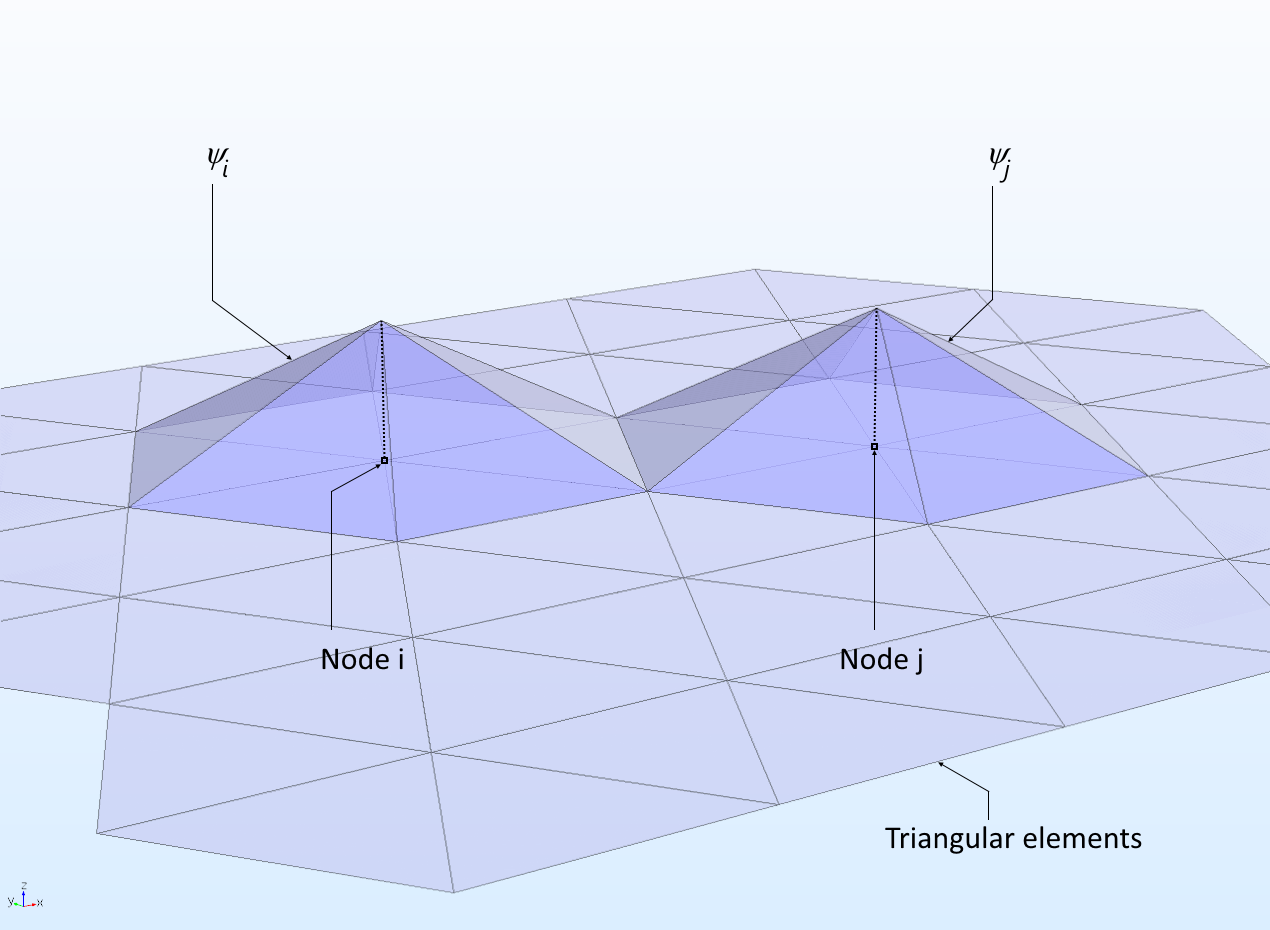
\includegraphics[width=\textwidth]{figures/triangle_overlap_1}
    \end{subfigure}
    \begin{subfigure}{0.49\linewidth}
        \centering
        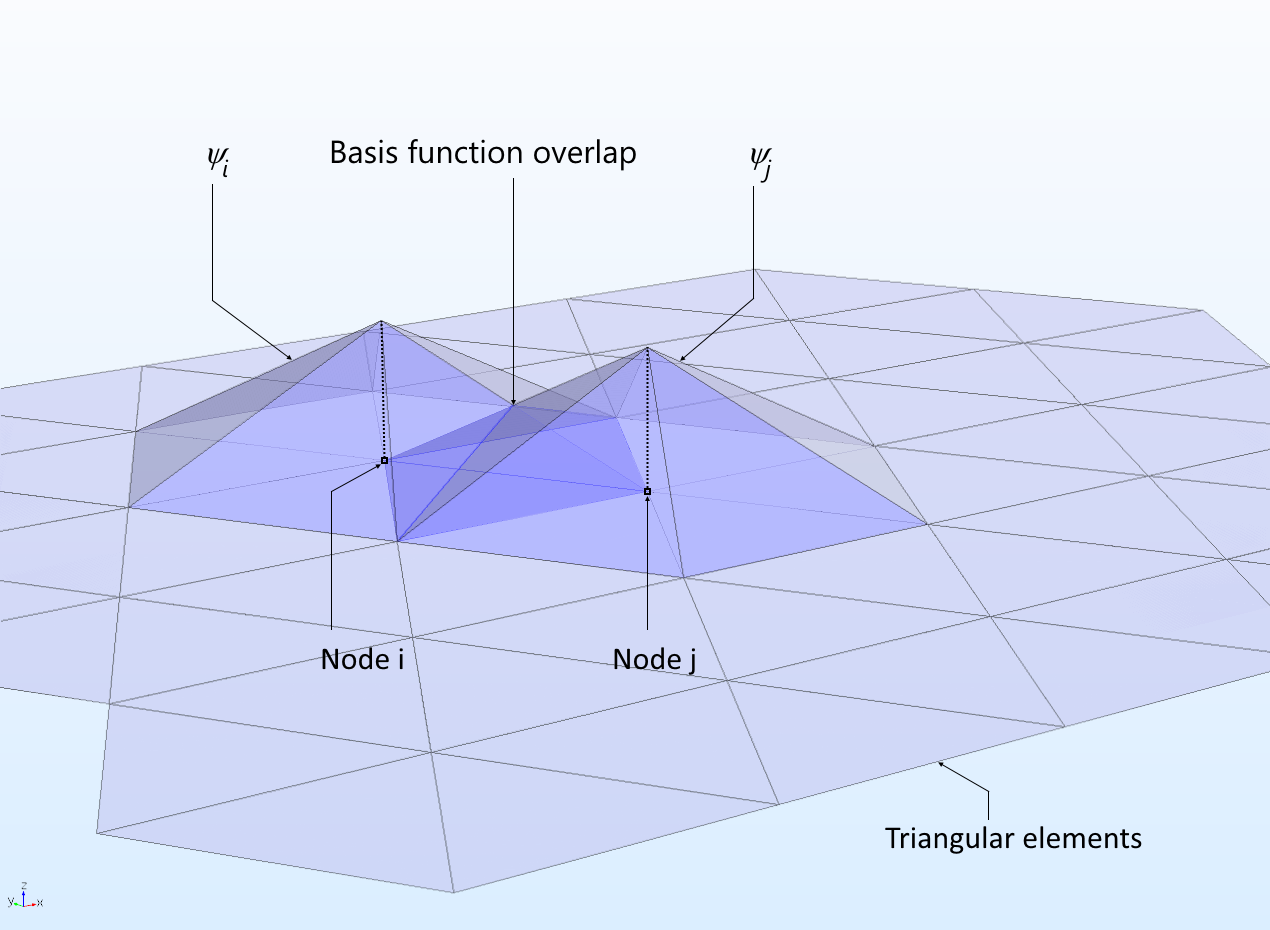
\includegraphics[width=\textwidth]{figures/triangle_overlap_2}
    \end{subfigure}
    \caption{Only neighboring points have overlapping basis functions. Image taken from
        \href{https://www.comsol.com/multiphysics/finite-element-method}{the COMSOL website}.}
    \label{fig:triangle_overlap}
\end{figure}

For the derivative term, first, we approximate $\hat{\vb{v}}(\vb{k})$ as a piecewise constant
unit vector field normal to each triangle. That is,
\begin{equation}
\hat{\vb{v}}(\vb{k}) = \text{sgn}(i,j,k) \vu{n}(i,j,k); \quad
\vb{n}(i,j,k) \equiv (\vb{k}_j - \vb{k}_i) \times (\vb{k}_k - \vb{k}_i),
\end{equation}
where $\hat{\vb{n}} = \vb{n}/\norm{\vb{n}}$ and $\text{sgn}(i,j,k) = \pm1$ is chosen such that
the normals always point outwards from the surface.
Also note that $\norm{\vb{n}(i,j,k)} = \alpha(i,j,k)$. The other term we need is gradient of
$\psi_j$ on triangle $T(i,j,k)$. Since $\psi_j$ is linear on this triangle and peaks at $j$,
its gradient is a constant vector pointing to $j$ and perpendicular to the opposite edge
$\vb{k}_k - \vb{k}_i$.
\begin{equation}
\grad_{\vb{k}} \psi_j(\vb{k}) = \frac{\vb{u}_j(i,j,k)}{u^2_j(i,j,k)};
\end{equation}
where $u_j(i,j,k) = \norm{\vb{u}_j(i,j,k)}$ and
\begin{equation}
\vb{u}_j(i,j,k) = (\vb{k}_j - \vb{k}_i)
- \frac{(\vb{k}_j-\vb{k}_i)\vdot(\vb{k}_k-\vb{k}_i)}{\abs{\vb{k}_k - \vb{k}_i}^2}
(\vb{k}_k - \vb{k}_i).
\end{equation}
The vector $\vb{u}_j(i,j,k)$ is obtained by projecting the vector $\vb{k}_j - \vb{k}_i$ onto the
direction perpendicular to the edge $\vb{k}_k - \vb{k}_i$. This is done by subtracting the component
in the direction of $\vb{k}_k - \vb{k}_i$ from $\vb{k}_j - \vb{k}_i$. Using these calculations, we
can finally compute the derivative term.
\begin{equation}
    \qty(\hat{\vb{v}}(\vb{k})\cross\vu{B})\vdot\grad_{\vb{k}}\psi_j
    = \qty(\grad_{\vb{k}}\psi_j\cross\hat{\vb{v}}(\vb{k}))\vdot\vu{B}
    = \text{sgn}(i,j,k)\qty(\frac{\vb{u}_j(i,j,k)\cross\vu{n}(i,j,k)}{u^2_j(i,j,k)})\vdot\vu{B}.
\end{equation}
You can simplify this expression by hand. But, using a bit of geometric thinking, it can be done
in a simpler way: since $\vb{u}_j$ is perpendicular to $\vb{k}_i - \vb{k}_k$ and $\vu{n}$ is
perpendicular to the plane of the triangle such that it is generated by counterclockwise
("right-handed") cross products of vectors on the plane, $\vb{u}_j\cross\vu{n}$ must be in the
direction of $\vb{k}_i - \vb{k}_k$. This means
\begin{equation}
    \vb{u}_j(i,j,k)\cross\vu{n}(i,j,k) = u_j(i,j,k)
    \frac{\vb{k}_i-\vb{k}_k}{\norm{\vb{k}_i-\vb{k}_k}}.
\end{equation}
Furthermore, $u_j(i,j,k)$ and $\vb{k}_i - \vb{k}_k$ can be taken as the high and the base of
the triangle $T(i,j,k)$ respectively, so the product of their norms is twice the area of the
triangle, which is the same as the Jacobian $\alpha(i,j,k)$. Putting it all together, we have
\begin{equation}
    \qty(\hat{\vb{v}}(\vb{k})\cross\vu{B})\vdot\grad_{\vb{k}}\psi_j
    = \frac{\text{sgn}(i,j,k)}{\alpha(i,j,k)}(\vb{k}_i-\vb{k}_k)\vdot\vu{B}.
\end{equation}
Using this, we can compute the derivative matrix.
\begin{align}
    (D_{\vu{v}\cross\vu{B}})_{ij} &= \int\dd{\vb{k}}\psi_i(\vb{k})
    \qty(\vu{v}(\vb{k})\cross\vu{B})\vdot\grad_{\vb{k}}\psi_j(\vb{k}) \\
    &= \sum_{(i,j,k) \in T_i \cap T_j}\alpha(i,j,k) \int_T\dd{x}\dd{y}(1-x-y)
    \frac{\text{sgn}(i,j,k)}{\alpha(i,j,k)}(\vb{k}_i - \vb{k}_k)\vdot\vu{B} \notag \\
    &= \frac{1}{6} \sum_{(i,j,k) \in T_i \cap T_j}\text{sgn}(i,j,k)(\vb{k}_i-\vb{k}_k)\vdot\vu{B}.
    \notag
\end{align}
Note that this matrix is antisymmetric and the elements on the main diagonal are equal to zero.
The antisymmetry is apparent from the $\text{sgn}(i,j,k)$ term. The diagonal being zero is a bit
more subtle. Think about what the sum means when $i=j$. We are summing the edges not containing
the point $i$ over all triangles containing $i$. But, for any point inside a closed surface, this
just means going around the point $i$ in a closed loop. So, since we are concerned with closed
surfaces, this is always zero.

Finally, for the in-scattering term, we have
\begin{gather}
\Xi_{ijmn} = \qty(\int\dd{\vb{k}}\psi_i(\vb{k})\psi_m(\vb{k}))
    \qty(\int\dd{\vb{k'}}\psi_j(\vb{k'})\psi_n(\vb{k'})) = M_{im} M_{jn} \\
S_{ij} = \sum_{m,n}\Xi_{ijmn}s^{mn} = \sum_{mn}M_{im}M_{jn}s^{mn}.
\end{gather}

In summary, defining
\begin{empheq}[left=\empheqlbrace]{align}
    \alpha_i &= \sum_{(i,j,k) \in T_i} \alpha(i,j,k), \\
    \alpha_{ij} &= \sum_{(i,j,k) \in T_i \cap T_j} \alpha(i,j,k), \\
    \vb{d}_{ij} &= \sum_{(i,j,k) \in T_i \cap T_j} \text{sgn}(i,j,k)(\vb{k}_i - \vb{k}_k),
\end{empheq}
the different matrices can be expressed as
\begin{gather}
    M_{ij} = \frac{\alpha_i}{12}\delta_{ij} + \frac{\alpha_{ij}}{24}\delta_{\expval{ij}}, \\
    \Gamma_{ij} = \qty(\frac{\alpha_i\gamma^i}{20}
        + \sum_k\frac{\alpha_{ik}\gamma^k}{60}\delta_{\expval{ik}})\delta_{ij}
        + \qty(\frac{\alpha_{ij}}{60}(\gamma^i+\gamma^j) + \sum_k\frac{\alpha(i,j,k)\gamma^k}{120}
            \delta_{\expval{ik}}\delta_{\expval{jk}})\delta_{\expval{ij}}\\
    (D_{\vu{v}\cross\vu{B}})_{ij} = \frac{1}{6}\vu{B}\vdot\vb{d}_{ij}\delta_{\expval{ij}}. \\
    S_{ij} = \frac{\alpha_i\alpha_j}{12}s^{ij} + \alpha_i\sum_n\alpha_{jn}s^{in}\delta_{\expval{jn}}
    + \alpha_j\sum_m\alpha_{im}s^{mj}\delta_{\expval{im}}
    + \sum_{m,n}\alpha_{im}\alpha_{jn}s^{mn}\delta_{\expval{im}}\delta_{\expval{jn}}.
\end{gather}
$\delta_{\expval{ij}}$ is equal to 1 if $i$ and $j$ are neighboring points, and 0 otherwise.
Technically, due to the definitions, it is not really needed, but I include it to make things
a bit clearer.

\section{Implementation Details}
\subsection{Solving Matrix Equations}
When sticking with the relaxation time approximation and ignoring the in-scattering,
the matrices are sparse, since there is only overlap between neighboring elements.
Even better, they are nearly \emph{banded}, meaning that the nonzero elements are only on the main
diagonal and the minor diagonals surrounding it. I say nearly, because there are also extra corner
terms, coming from the periodic boundary conditions of the Brillouin zone.

For solving our matrix equations which involve nearly-banded matrices, there are two approaches.
The first is to treat the matrix as a general sparse matrix and utilize sparse matrix solvers.
The second approach is to use a banded matrix solver in combination with some other method for
handling the off-diagonal, periodic boundary terms.

In terms of time complexity, efficient sparse matrix solvers achieve
$\mathcal{O}(N^{3/2})$ performance, where $N$ indicates the number of nonzero elements in the
matrix. In our systems, since the nonzero elements correspond to single-point terms and terms
coming from the interaction of closest neighbors (which do not grow with the size of the system),
$N$ scales linearly with the number of discretization points of the system. Note that this is only
true when there is no in-scattering, since that term generates fully dense matrices, because of
the global interaction of states that the scattering Kernel introduces.

For a banded matrix solver, the time complexity is $\mathcal{O}(Nb^2)$ where $b$ is the
\emph{bandwidth} of the matrix, which is defined as the number of nonzero diagonals. So, whether
this beats the sparse solver depends on the scaling of the bandwidth. For a 2D system, this
bandwidth is constant and equal to 3, so our system is just a tridiagonal matrix, with 2 corner
terms coming from the endpoints of the closed Fermi surface interacting with each other. This
is extremely fast to solve, and thoroughly beats a sparse solver. However, for 3D systems, no
matter how we index the points, the bandwidth of the matrix is about $\sqrt{N}$ and the time
complexity will be around $\mathcal{O}(N^2)$, which is a worse scaling than the sparse solver.

To understand the 3D bandwidth scaling, picture a cylindrical surface. Imagine that to construct
this surface, we stack rings of points on top of each other. To index the points, we number the
points in each ring in order, and then move to the next layer. Each point, in addition to being
neighbors with points that have close index numbers, is also neighbors with a point from the
other end of the loop and also points from the top and bottom rings. The difference of the index
of these other points from the point is around the number of points in a ring. Since there are
$N$ points in total on the surface, the number of points in each of the rings should be around
$\sqrt{N}$. The nonzero elements are belong to neighbors, and now we have neighbors that have
indices that are $\sqrt{N}$ apart. On the matrix, this is a point where row number and the column
number (which correspond to two different points) are $\sqrt{N}$ apart, which means that it is
$\sqrt{N}$ away from the main diagonal. So, the bandwidth will be around $2\sqrt{N}$.

In practice, we see that the sparse solver is faster than the banded solver for any system size,
not just large systems. See Figure \ref{fig:sparse_vs_banded}. So, I decided to use a sparse
solver in general.

\begin{figure}
    \centering
    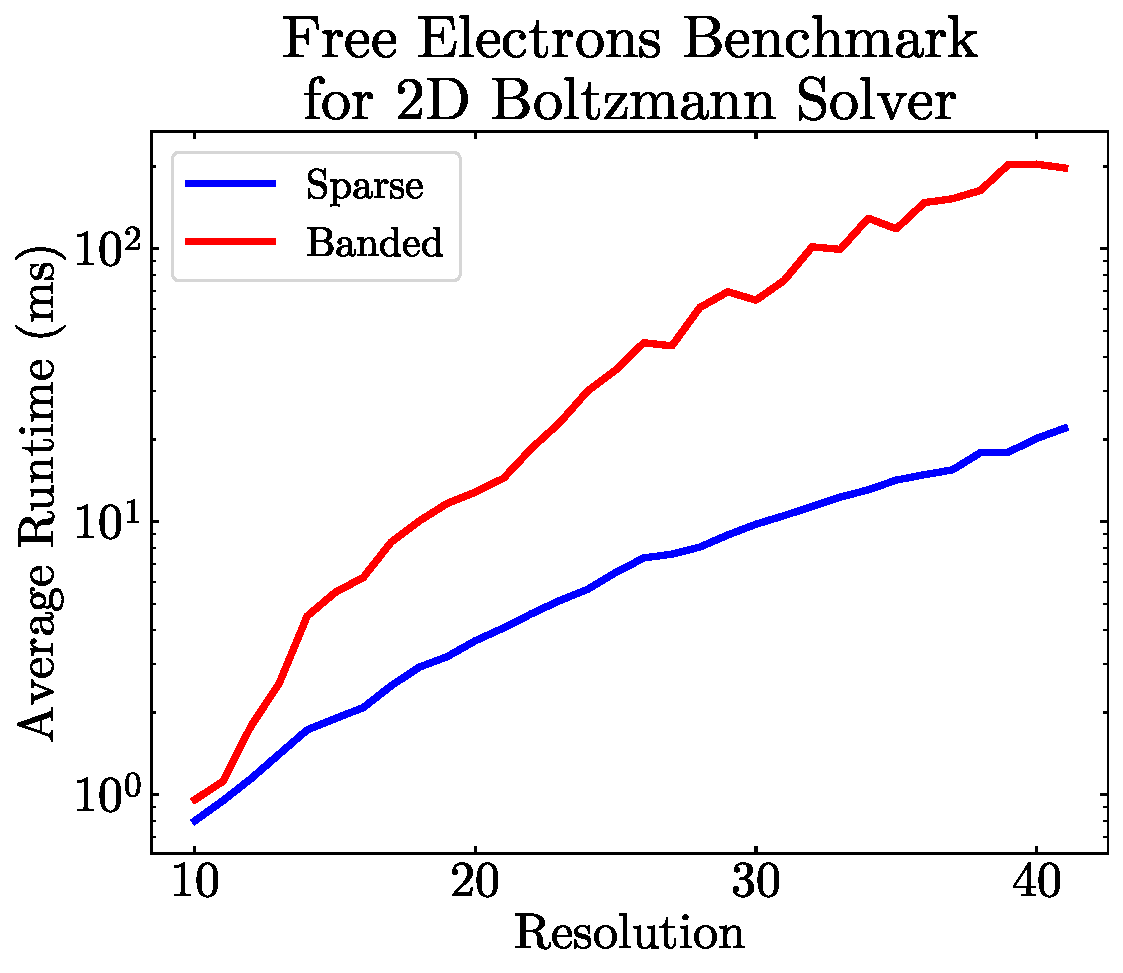
\includegraphics[width=0.7\textwidth]{figures/sparse_vs_banded}
    \caption{Comparison of the runtime of the sparse and banded implementations on a wide range of
        system sizes. The banded solver is never faster.}
    \label{fig:sparse_vs_banded}
\end{figure}

\subsection{Triangulation and Periodic Boundary Conditions}
There are many different ways of dividing up the Fermi surface into triangles. I tried any of these
triangulation methods that I could find, and I found that there is negligible difference between
them. So, in the package, the simplest one is used, which is \emph{marching cubes}. This was
already used before in the Chambers package.

One difference of the FEM and the Chambers formula is the fact that in the FEM, the periodic
boundary conditions of the Brillouin zone need to be enforced explicitly. This is only required
if we have a Fermi surface that crosses the boundaries of the Brillouin zone, and the symmetry
is broken in the axis where the crossing happens. So, for example, in the case of ADMR, where
we have a rotating field, pointing in arbitrary directions.

To enforce the periodic boundary conditions, we first assume the triangulated Fermi surface
has identical points on the opposite sides of the Brillouin zone on the axis where the crossing
happens. Then, to force these points to be the same in the solution, we reduce the system to
a smaller one with only unique points. Suppose we have some vector $\vb{b}$ where we have a
quantity attributed to each point on the full triangulated Fermi surface. Now, the same quantity
defined only on the unique points can be represented by a vector with smaller number of dimensions,
$\vb{b'}$. To go from $\vb{b}$ to $\vb{b'}$, we can define a matrix $P$ such that
\begin{equation}
    \vb{b'} = P\vb{b} \implies \vb{b} = P^T\vb{b'}.
\end{equation}
Most of the columns in $P$ just contain a single $1$, but for the points that are duplicated,
the corresponding column contains multiple $1$s, one for each duplicate point. Now, if we have
a matrix equation such that
\begin{equation}
    A\vb{x} = \vb{b}
\end{equation}
and we want the quantity
\begin{equation}
    \sigma = \vb{a}\vdot\vb{x} = \vb{a}\vdot\qty(A^{-1}\vb{b}),
\end{equation}
we can rewrite everything in the ``reduced'' space as
\begin{equation}
    A\vb{x} = P^T\vb{b'} \implies \sigma = P^T\vb{a'}\vdot\qty(A^{-1}P^T\vb{b'}).
\end{equation}
One might prefer to think of $P$ as a transformation for the matrix $A$:
\begin{equation}
    \sigma = \vb{a}^T\vb{x} = \vb{a'}^T P A^{-1} P^T \vb{b'} = \vb{a'}^T (P A P^T)^{-1} \vb{b'}, 
\end{equation}
but I like to keep it as a transformation for the vectors, since we can just transform the vectors
and keep every other step the same. In fact. the transformation only needs to be done once, since
$\vb{a}$ and $\vb{b}$ are different components of the projected velocity $\vb{v}_i$ and $\vb{v}_j$,
and it suffices to transform the matrix containing each component in each column. This turns out
to be faster than transforming the matrix $A$.

\textbf{Note:} In the code, $P^T$ is called the projection matrix and is all that the package works
with, since it is the only thing that is needed to transform the vectors. You can think of $P^T$
as the transformation reducing the full space to the unique space. The reason I did not use this
for the explanation is that it is not clear that the reduced space point should be a sum of the
full space points before seeing the transformation matrix from the reduced space to the full space.

\subsection{Curvature corrections}
There is one very cheap correction we can do to improve the accuracy at low resolutions. When
triangulating a curved surface, we are always underestimating the surface area, since the flat
triangles always have less surface area than the patch on the curved surface that they are
approximating. This happens when the points are on the surface. Now, imagine having the
triangular faces tangent to the surface instead. In this case, the surface area is much closer
to the actual curved surface. In the limit, these two approximations converge to the same
surface, but at low resolutions, the tangent plane approximates the surface area much better.
To understand this intuitively, imagine taking a curved patch of the surface and flattening it
on a table. The resulting shape is the projection of the curved patch onto the tangent plane.
This looks close to the tangent face we are using, but slight misalignments make it inexact.
But it is still much better than the face that has the vertices on the surface.

\section{Results}
\subsection{Free Electrons}
Figure \ref{fig:free_electrons} shows the comparison of the FEM to the Drude model for free
electrons in two dimensions. As expected, they match perfectly. The convergence is exponential,
as seen in Figure \ref{fig:free_electrons_error}. The results are quite similar in 3D,
so I do not include them here.
\begin{figure}%[h]
    \centering
    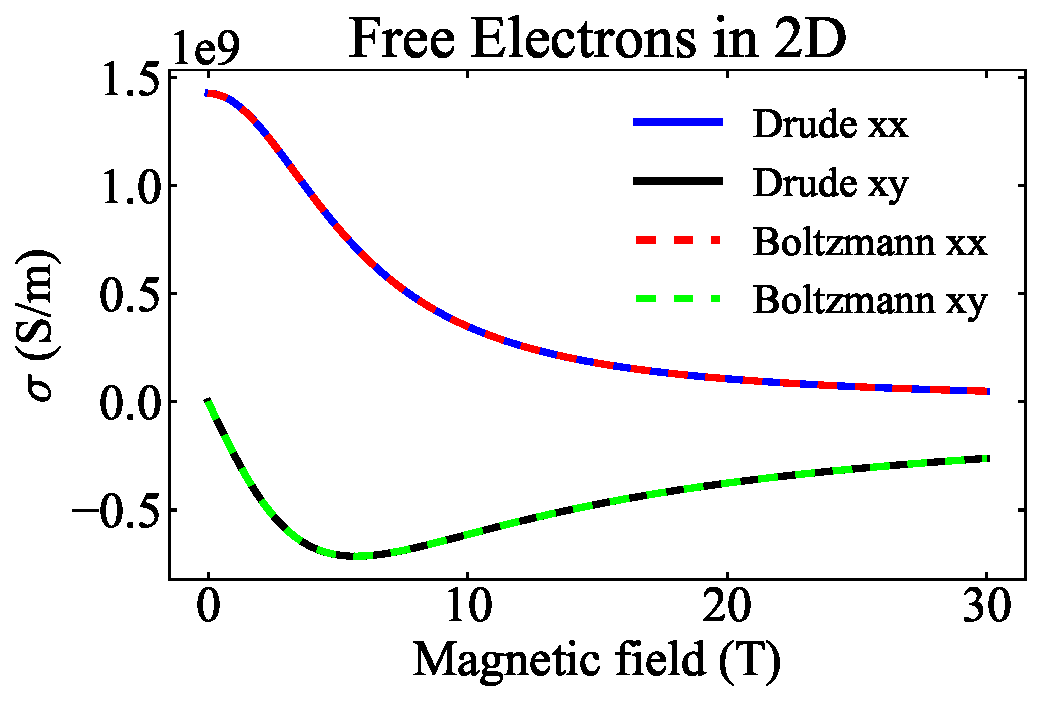
\includegraphics[width=0.7\textwidth]{figures/boltzmann_vs_drude_2d}
    \caption{Comparison of the FEM to the Drude model for free electrons in 2D at a relatively
        low marching cubes resolution of 20.}
    \label{fig:free_electrons}
\end{figure}
\begin{figure}%[h]
    \centering
    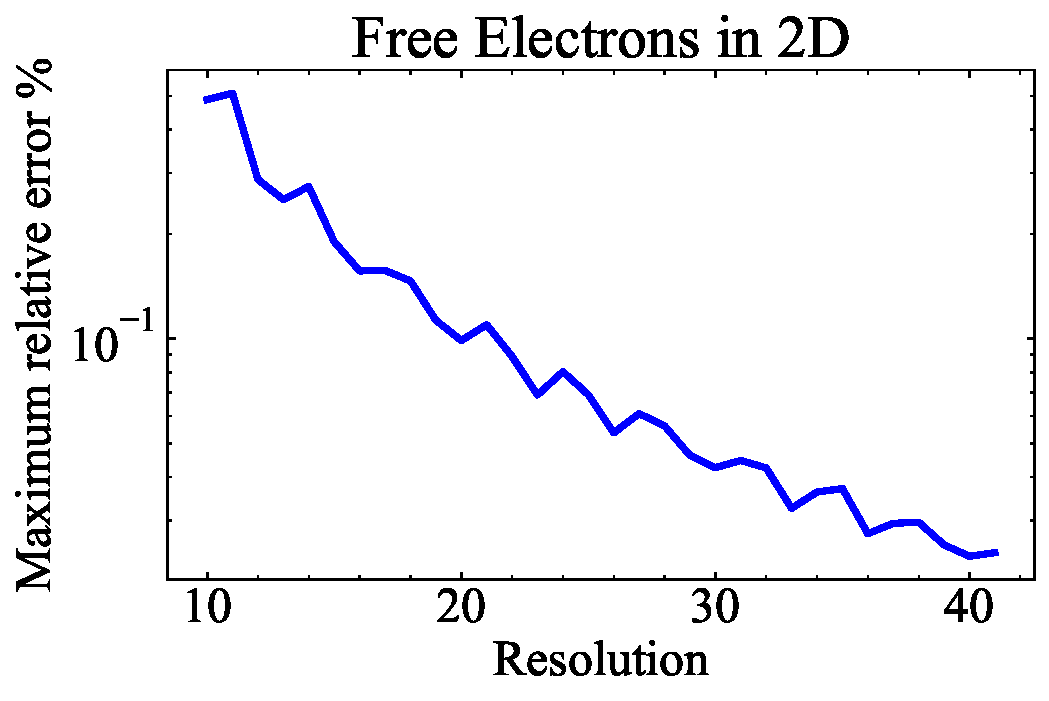
\includegraphics[width=0.7\textwidth]{figures/boltzmann_vs_drude_2d_error}
    \caption{The maximum relative error of the FEM compared to the Drude model for free
        electrons in 2D as a function of the marching cubes resolution. The convergence
        is exponential, and we already hit $99.9\%$ accuracy at a resolution of around 20.
        The jaggedness is because of imperfections in the triangulation.}
    \label{fig:free_electrons_error}
\end{figure}

\subsection{Cuprates}
In the more complicated case of the cuprates, we only have the Chambers formula to compare to.
Since the Chambers formula itself is an approximation, it is hard to evaluate the actual
accuracy of the FEM. However, seeing as the results of the FEM converge faster, and that the
results of Chambers get closer to the results of the FEM at higher resolutions we can be
confident that the FEM is more accurate. See Figure \ref{fig:fem_vs_chambers_admr} and
\ref{fig:fem_vs_chambers_resistivity} for some comparisons. See Figure
\ref{fig:fem_vs_chambers_convergence} for a comparison of the convergence. Also, you can see
from the comparison to the Drude model in Figure \ref{fig:free_electrons_resistivity} that the
FEM is more accurate at calculating the resistivity for free electrons, which adds to the
evidence that the FEM is more accurate.

\begin{figure}%[h]
    \centering
    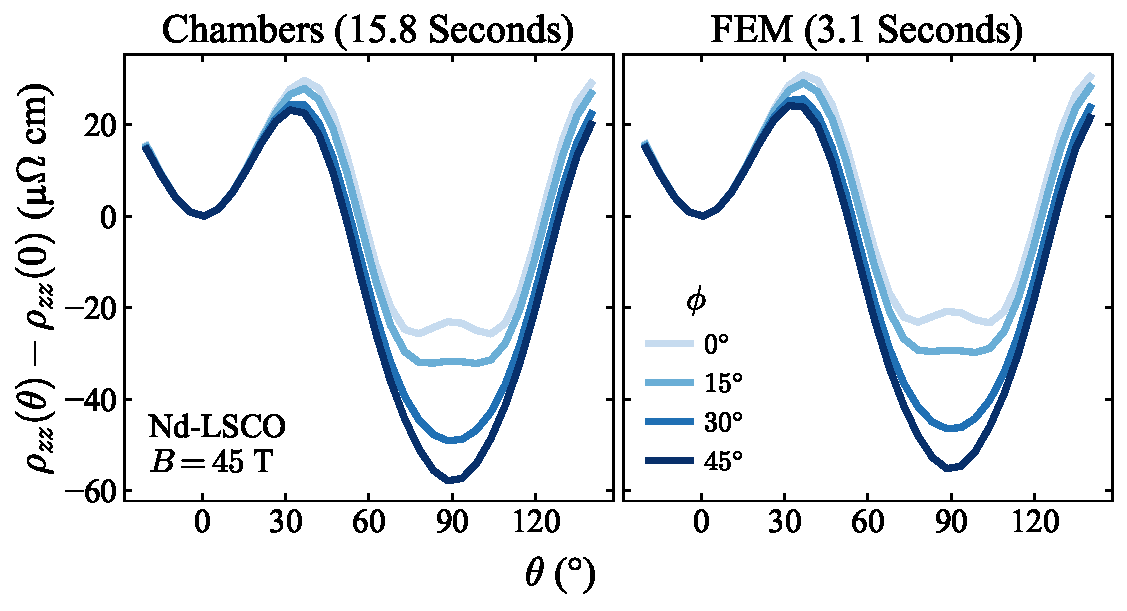
\includegraphics[width=\textwidth]{figures/fem_vs_chambers_admr}
    \caption{Comparison of the ADMR of Nd-LSCO calculated by the FEM and the Chambers formula.
        By focusing on the relative changes only instead of the full absolute resistivity, we
        can see that the models are quite similar.}
    \label{fig:fem_vs_chambers_admr}
\end{figure}
\begin{figure}%[h]
    \centering
    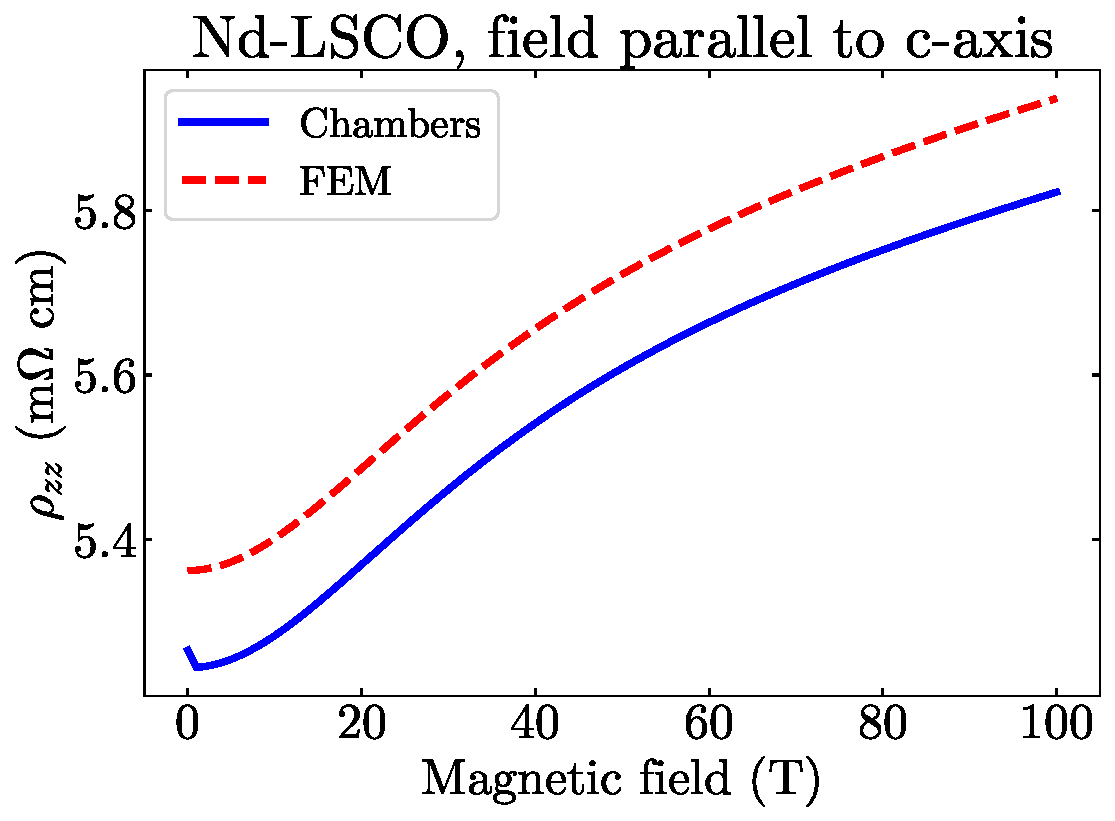
\includegraphics[width=0.7\textwidth]{figures/fem_vs_chambers_resistivity}
    \caption{Comparison of the magnetoresistance of Nd-LSCO calculated by the FEM and the
        Chambers formula. This is at high resolution, and there is even a larger discrepency
        at lower resolutions. However, most of the discrepency comes from a difference in the
        absolute value, and the relative changes are quite similar.}
    \label{fig:fem_vs_chambers_resistivity}
\end{figure}
\begin{figure}
    \centering
    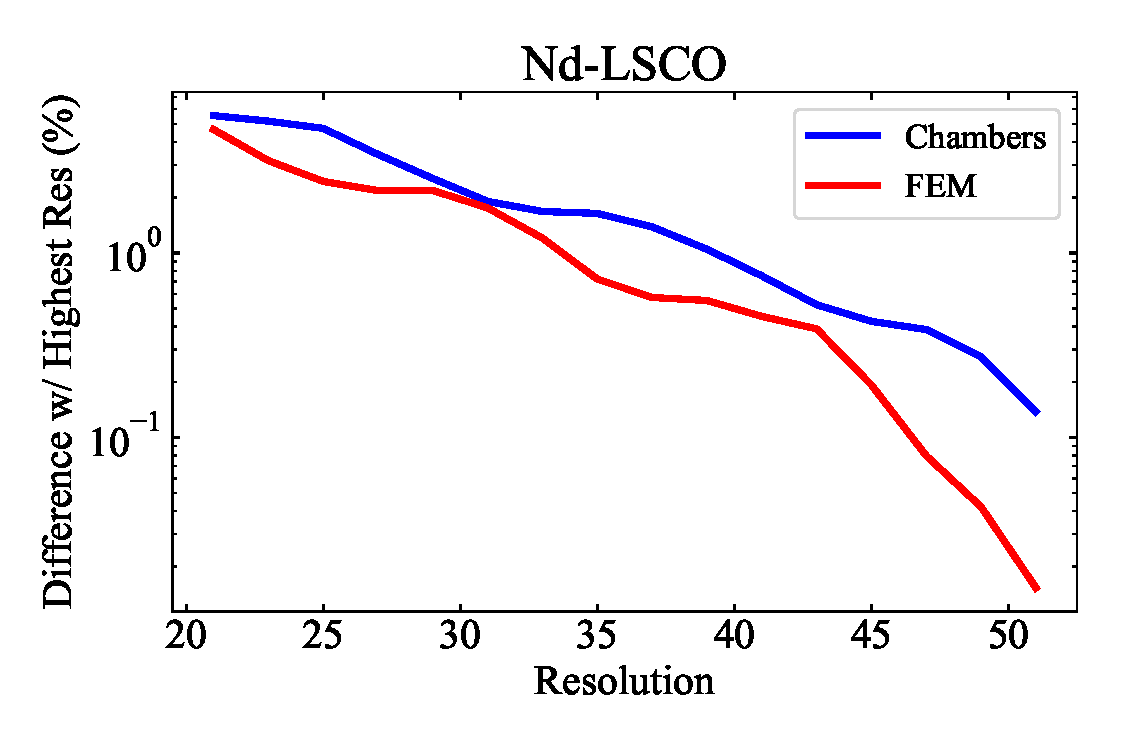
\includegraphics[width=0.7\textwidth]{figures/fem_vs_chambers_convergence}
    \caption{The convergence of the FEM and the Chambers formula for Nd-LSCO. As you can see,
        the FEM converges faster, which indicates that it is probably more accurate.}
    \label{fig:fem_vs_chambers_convergence}
\end{figure}
\begin{figure}%[h]
    \centering
    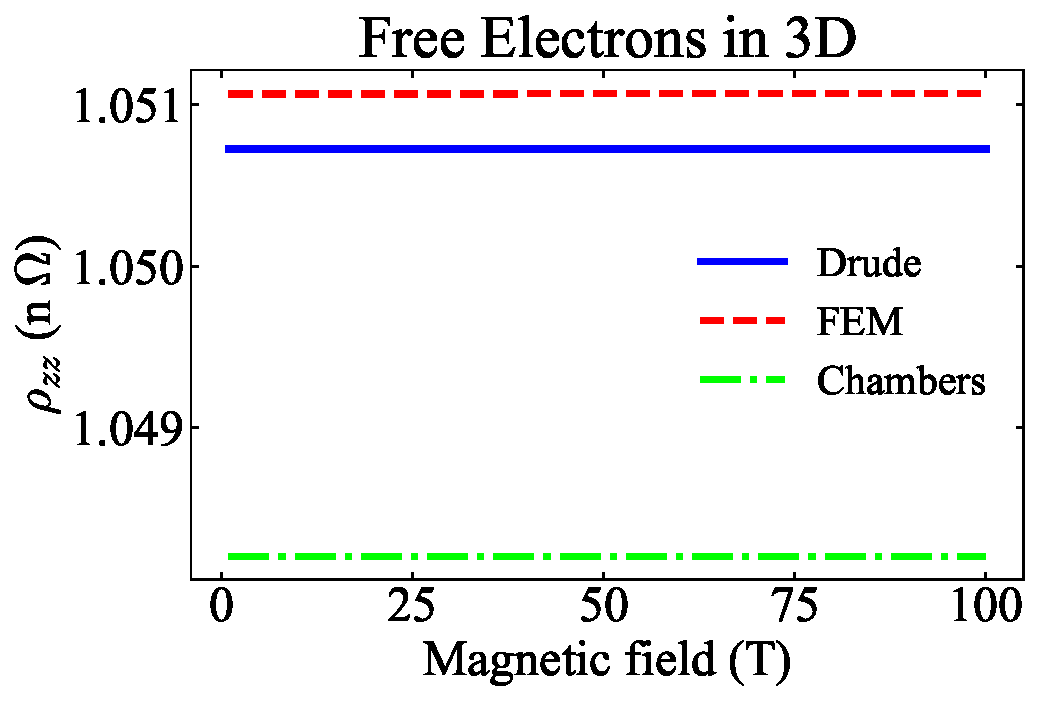
\includegraphics[width=0.7\textwidth]{figures/free_electrons_resistivity}
    \caption{The resistivity of free electrons is 3D, as calculated by the FEM and the
        Chambers formula (with similar resolutions), compared to the Drude model that is the
        exact solution here. As you can see, the FEM is more accurate.}
    \label{fig:free_electrons_resistivity}
\end{figure}

We can also see that the $R_H$ of the FEM correctly converges to $-1/ne$ at very high fields.
See Figure \ref{fig:fem_vs_chambers_rh}. This does not require high resolutions, and higher
fields do not require more computation, unlike the Chambers formula. This shows another
advantage of the FEM over the Chambers formula.

\begin{figure}%[h]
    \centering
    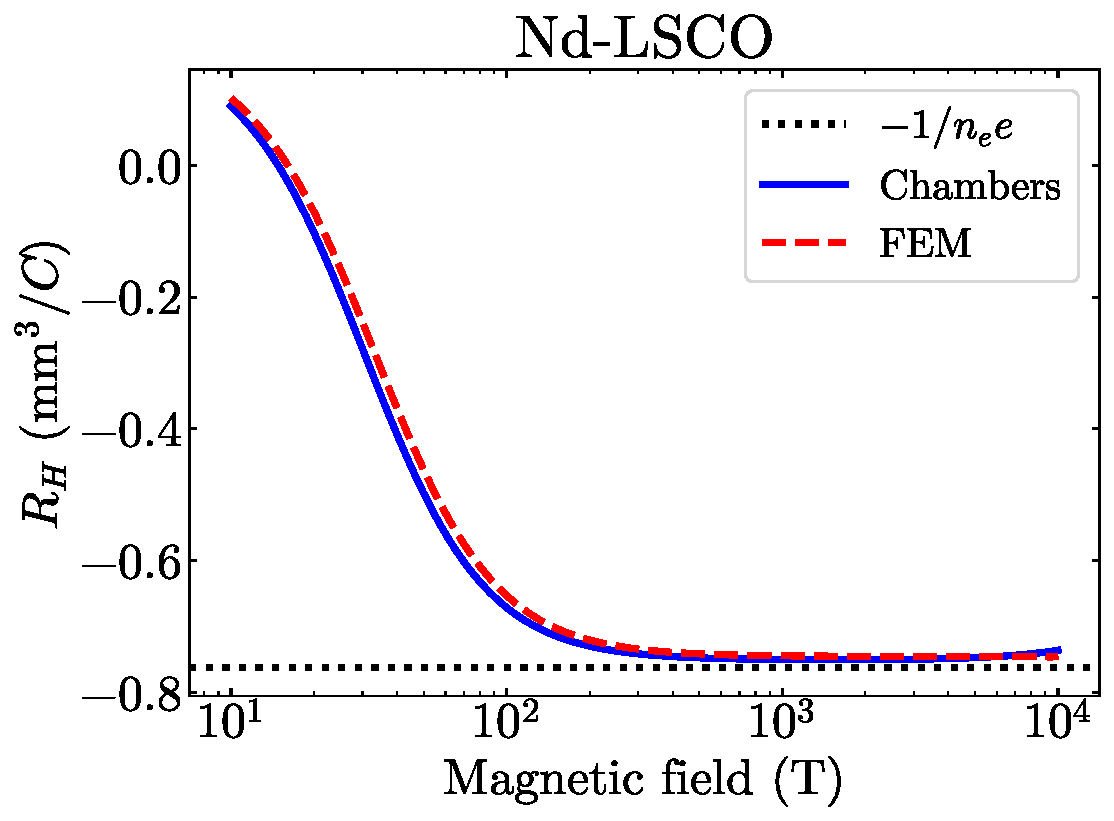
\includegraphics[width=0.7\textwidth]{figures/fem_vs_chambers_rh}
    \caption{The Hall coefficient of Nd-LSCO calculated by the FEM and the Chambers formula.
        Both correctly converge to $-1/ne$ at high fields.}
    \label{fig:fem_vs_chambers_rh}
\end{figure}

\subsection{Performance}
As seen in Figure \ref{fig:fem_vs_chambers_admr} from the previous section, the FEM is 5 to 6
times faster than the Chambers formula at resolutions with similar accuracy. Keep in mind that
this is a comparison to the marching squares implementation, which is faster but not always
possible to use, as the absolute value of the resistivity can be quite inaccurate.

Having said that, the true power of the FEM becomes apparent in cleaner materials like PdCoO$_2$.
The FEM can be two orders of magnitude faster. For an example, see Figure
\ref{fig:fem_vs_chambers_pdcoo2}.

\begin{figure}
    \centering
    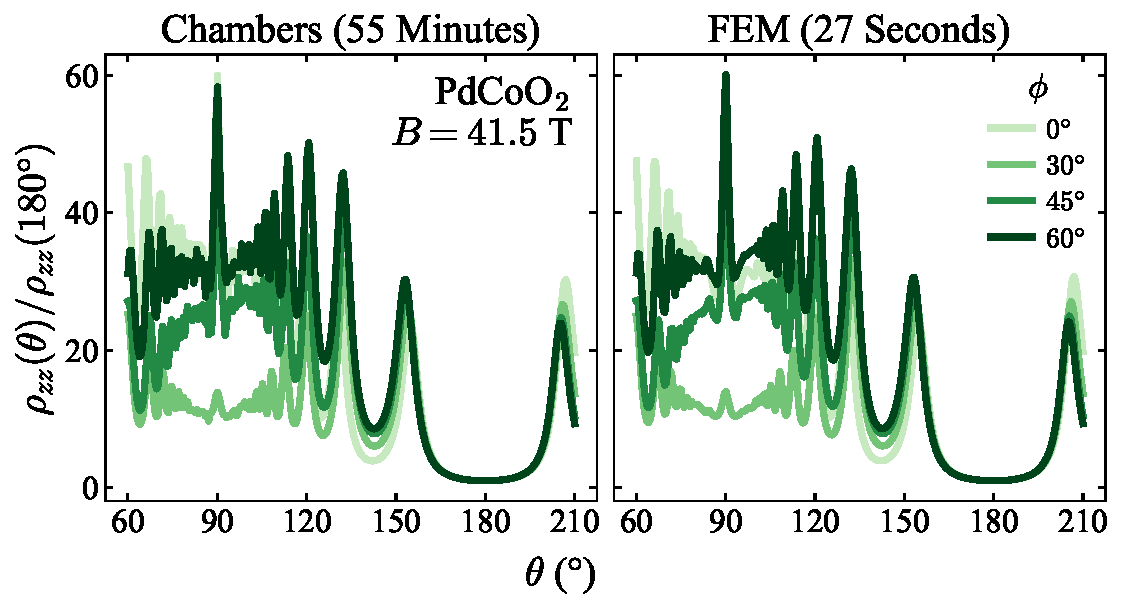
\includegraphics[width=\textwidth]{figures/fem_vs_chambers_pdcoo2}
    \caption{Comparison of the ADMR of PdCoO$_2$ calculated by the FEM and the Chambers
        formula. The FEM is more than 120 times faster at similar accuracy.}
    \label{fig:fem_vs_chambers_pdcoo2}
\end{figure}
\end{document}
